\section{Computational Design}

The main idea of this chapter is to use models and algorithms to help design and optimize interfaces. The chapter will contain: 

\begin{itemize}[itemsep=-5pt, topsep=0pt, leftmargin=*]
	\item Modeling task as combinatorial optimization problem
	\item User models as cost / goodness functions in optimization
	\item The assignment problem and applications in HCI
	\item Examples
\end{itemize}

Example: 50 different items yield 50! options to create menus. 

\smallskip

\textit{To evaluate a menu we can use:} \medskip

Time to move to an element $i$ :
$$t_i = a + b \log_2 \left( \frac{A_i}{W_i} + 1 \right)$$
Average time to operate a menu:
$$T = \sum_{i} p_i t_i$$

\textbf{Design as Search}

As a goal we want to find the best design decision for given objectives. \medskip

Some benefits of using algos in design: 


\begin{itemize}[itemsep=-5pt, topsep=0pt, leftmargin=*]
	\item Efficiently search large solution spaces
	\item Systematic, rigorous process
	\item Improved quality and reliability
	\item Guarantees for goodness of outcomes
\end{itemize}

We want to find optimal $x \in X$ where $X \in \mathbb{K}^n$ which maximizes $f(x)$. So $X$ is the set of all feasible solutions. \medskip

\textit{Formulate optimization problem}
 \begin{multicols}{2}
    \begin{itemize}[itemsep=-5pt, topsep=0pt, leftmargin=*]
        \item The design space (variables, constraints)
        \item Objective functionality
        \item Way to solve problem (solver)
    \end{itemize}
 \end{multicols}
    

\textit{Design Space} \smallskip

A combination of all design variables form the design space. Each variable represents an open decision (usually discrete):

\begin{itemize}[itemsep=-5pt, topsep=0pt, leftmargin=*]
	\item Boolean(e.g. show label)
	\item Integer(e.g. color)
	\item Categorical(e.g. type of element)
	\item Continous(e.g. color value)
\end{itemize}

As not all combinations yield a feasible design we need to introduce constraints. \medskip

Decision variables: \smallskip

$x_{ik} = 
\begin{cases} 
1, & \text{if command } i \text{ assigned to slot } k \\
0, & \text{otherwise}
\end{cases}$ \medskip

Design space: \smallskip

$X = \{ \mathbf{x} = (x_{ik}) \mid i,k = 1 \ldots N, x_{ik} \in \{0,1\} \}$ \medskip

\textit{Constraints (feasible space)}: \medskip

$\sum_{k=1}^{n} x_{ik} = 1 \quad \forall i = 1 \ldots N$, where each command is assigned to one slot. 


$\sum_{i=1}^{n} x_{ik} = 1 \quad \forall k = 1 \ldots N$, where each slot is assigned to one command.\medskip

\textit{Objective Function} \medskip

Assign a score the each solution in the design space. Goal is to find the solution that maximizes or minimizes the objective function.
Can be interpreted as quality indicator of UI. \smallskip

We can find an objective function in different ways.

\begin{itemize}[itemsep=-5pt, topsep=0pt, leftmargin=*]
	\item Math model
	\item Machine-learning model
	\item Simulation-based model
	\item Look up tables from empirical data
	\item Heristics, guidelines, best-practices
\end{itemize}

Example: Minimize average selection time (linear assignment problem):

$$\min \sum_{i=1}^{n} \sum_{k=1}^{n} p_{i} \cdot t_{k} \cdot x_{ik}$$
Where $p_i$ is prob of item $i$, $x_{ik}$ the constraints and $t_k$ the time to move to slot k from the top. \medskip

\textbf{Optimization Methods}

\textit{Mathematical, Exact Methods} \smallskip

Linear or (Mixed-) Integer Programming, Branch and Bound methods.

\begin{itemize}[itemsep=-5pt, topsep=0pt, leftmargin=*]
	\item + Explicit bounds and guarantees optimality
	\item + Fast standard solvers available
	\item - Objective function in closed mathematical form
	\item - Problem formulation might be hard to set up
\end{itemize}


\textit{Heuristic approximation algorithms} \smallskip

Simulated annealing, Genetic algorithms, Biology inspired algos

\begin{itemize}[itemsep=-5pt, topsep=0pt, leftmargin=*]
	\item + Programmatical description
	\item + Standard implementations available (Scipy, Opimization Toolbox Matlab etc.)
	\item + Flexible
	\item - No bounds or guarantees on global optimum
	\item - Can have many params
\end{itemize}


\textbf{Assignment Problem} \medskip

Assign items from Set A (e.g. menu items) to items in Set B (e.g. menu slots). \medskip

\textit{Quadratic Assignment Problem}

\begin{center}
	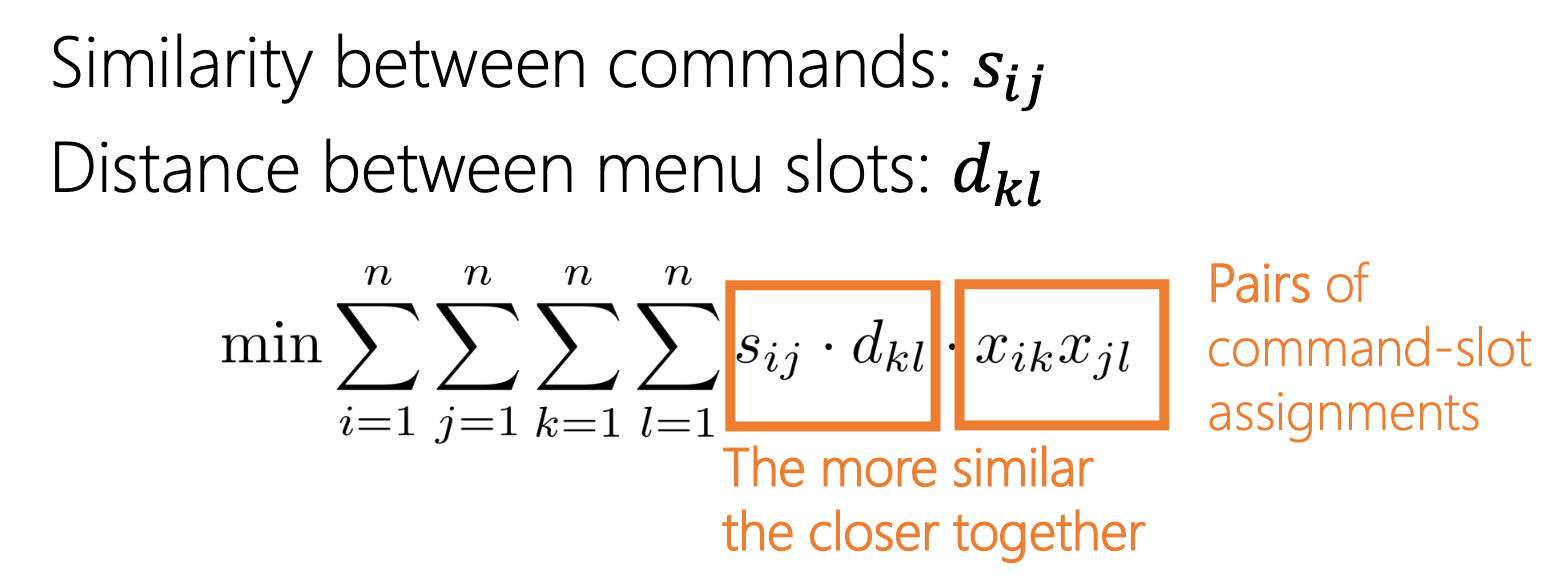
\includegraphics[width=\linewidth]{quadratic_assignment.png}
\end{center}

Is an np hard problem. Decision cost: $s_{ij} * d_{kl}$. The second part  $x_{ik} * x_{jl}$ is quadratic in the number of decisions. \medskip


\textbf{Example: The letter assignment problem} \smallskip

Question: Find best assignment of letters to keys on a smartphone to allow the fastest typing. 
Apply constraints: Each key assigned to exactly one letter, each letter assigned to exactly one key. 


\begin{center}
	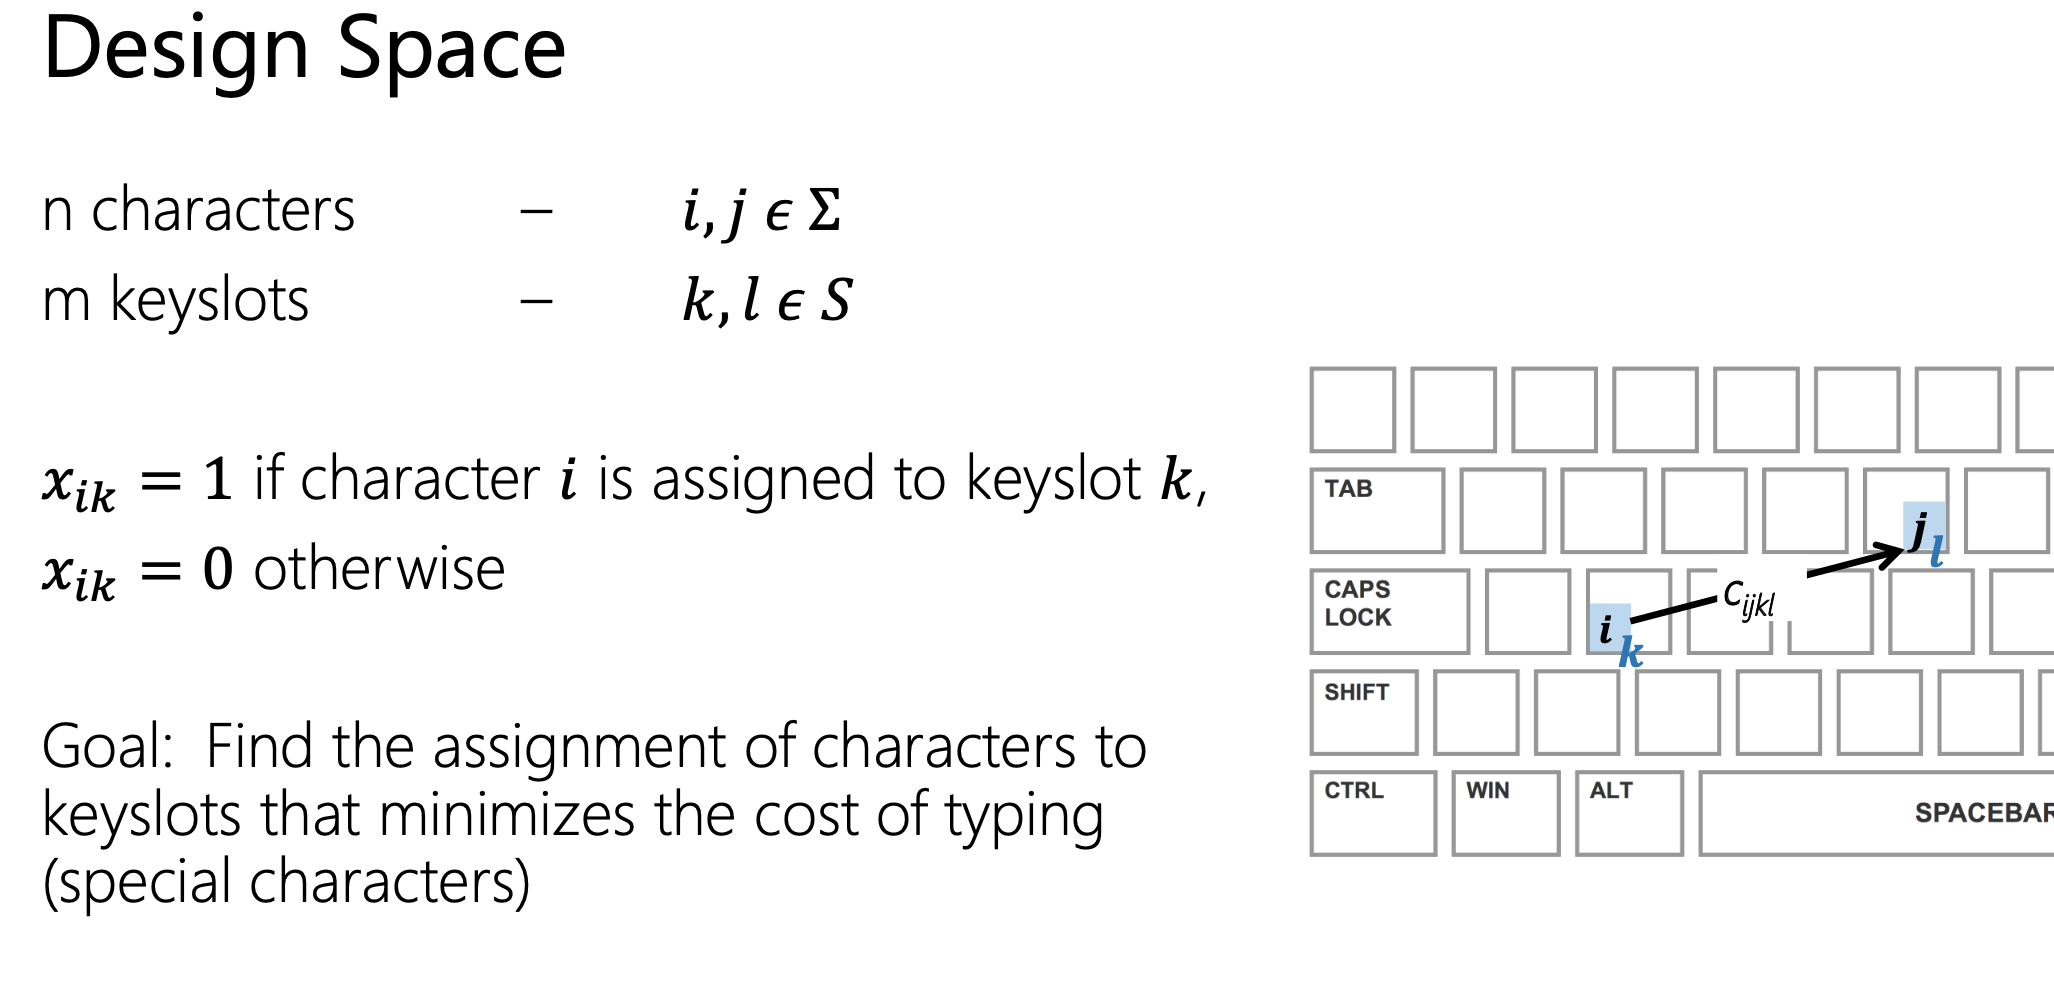
\includegraphics[width=\linewidth]{letter_example.png}
\end{center}

The goal was then to minimize the motor performance (average time to move between special characters and letters) and Ergonomics (minimize frequent extreme movements of wrist and fingers for special chars).
For Intuitiveness minimize the distance between similar special chars and also their visual similarity. Familiarity refers to redesign similar to known preferences. \medskip

\textbf{Multi-objective optimization} \smallskip

Goodness of user interface is determined by many aspects. 

\begin{itemize}[itemsep=-5pt, topsep=0pt, leftmargin=*]
	\item Performance
	\item Ergonomic and Fatigue
	\item Error prob.
	\item Mental workload
	\item Learnability
	\item Accessability
	\item Subjective experience
	\item etc. 
\end{itemize}


\begin{center}
	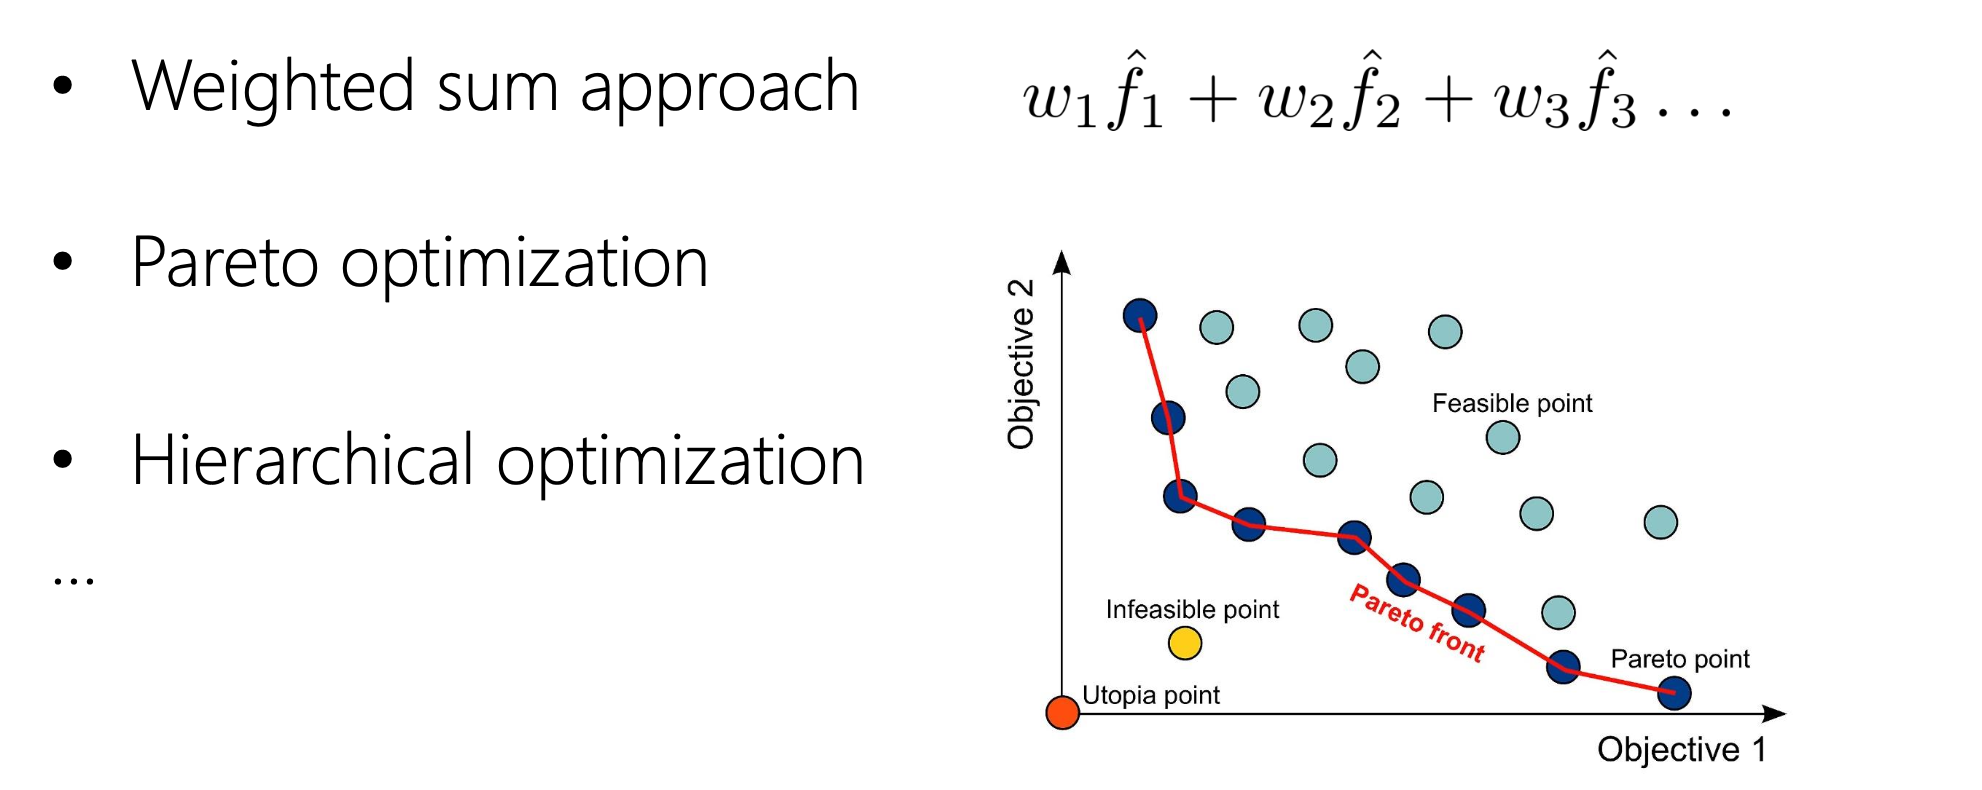
\includegraphics[width=\linewidth]{multi_objective.png}
\end{center}

\textbf{Combinatorial Optimization for User Interface Adaption} \smallskip

Optimize the UI to accomodate changes in environment, cognitive state, abilities, task, technical capabilities etc. Use different objectives such as optmize for quality and completeness. \smallskip

\textit{Element device compability}

\begin{center}
	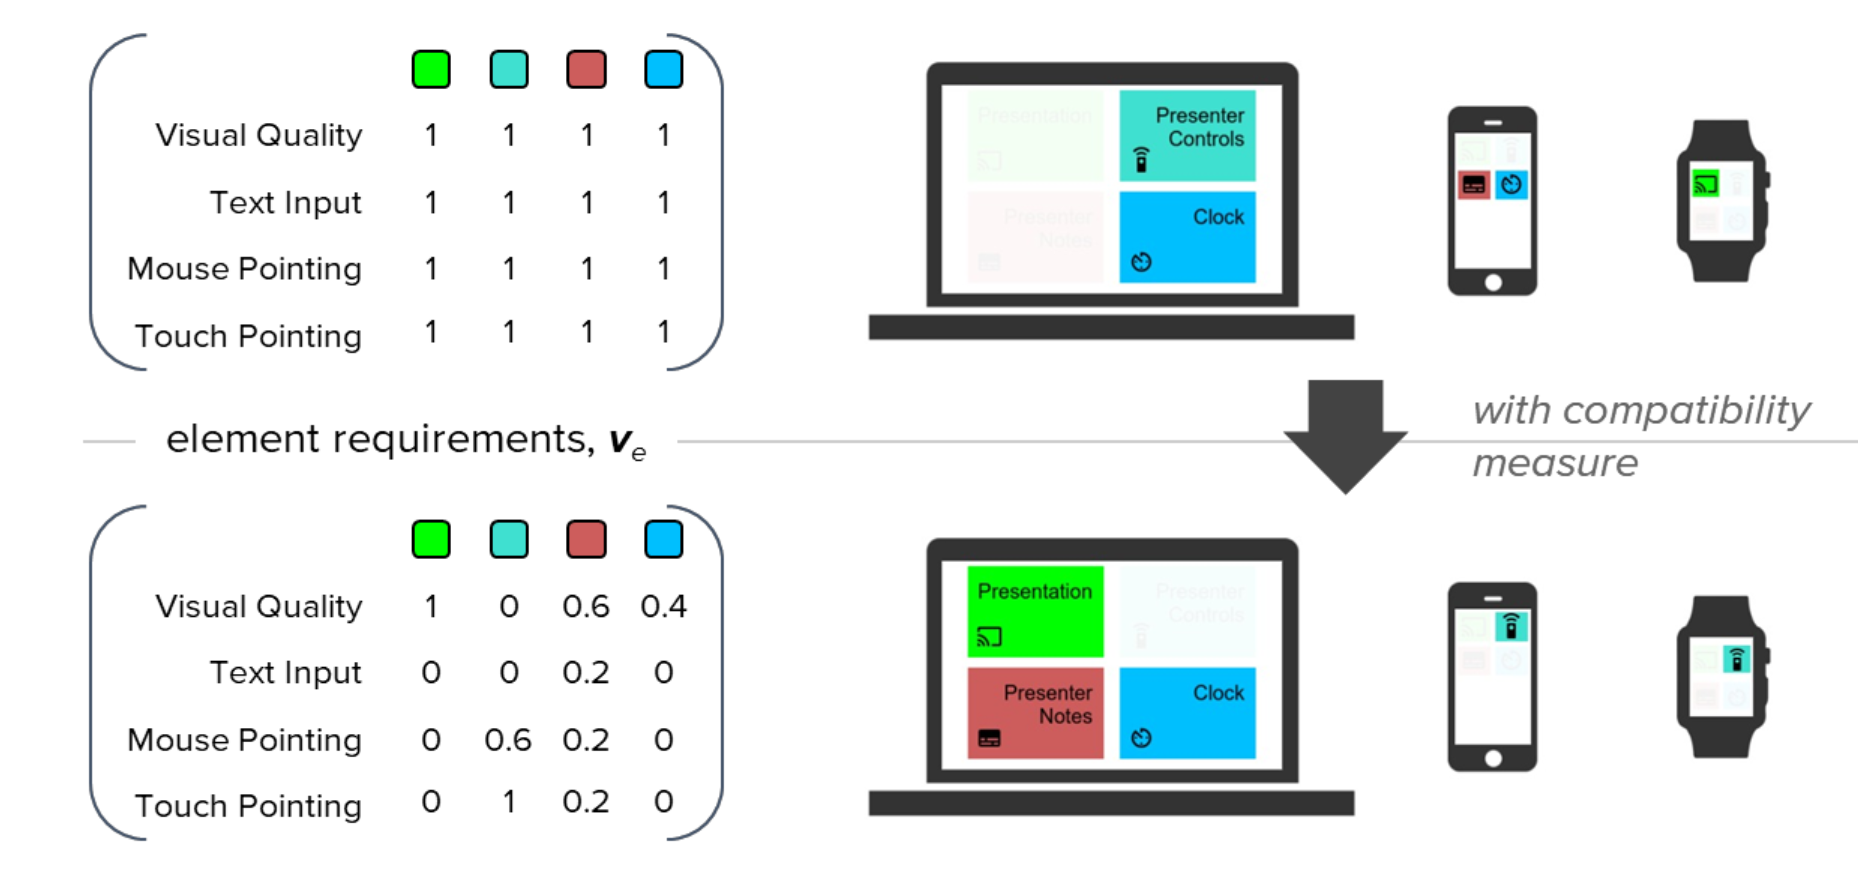
\includegraphics[width=\linewidth]{element_device_compability.png}
\end{center}

\textit{User roles}

\begin{center}
	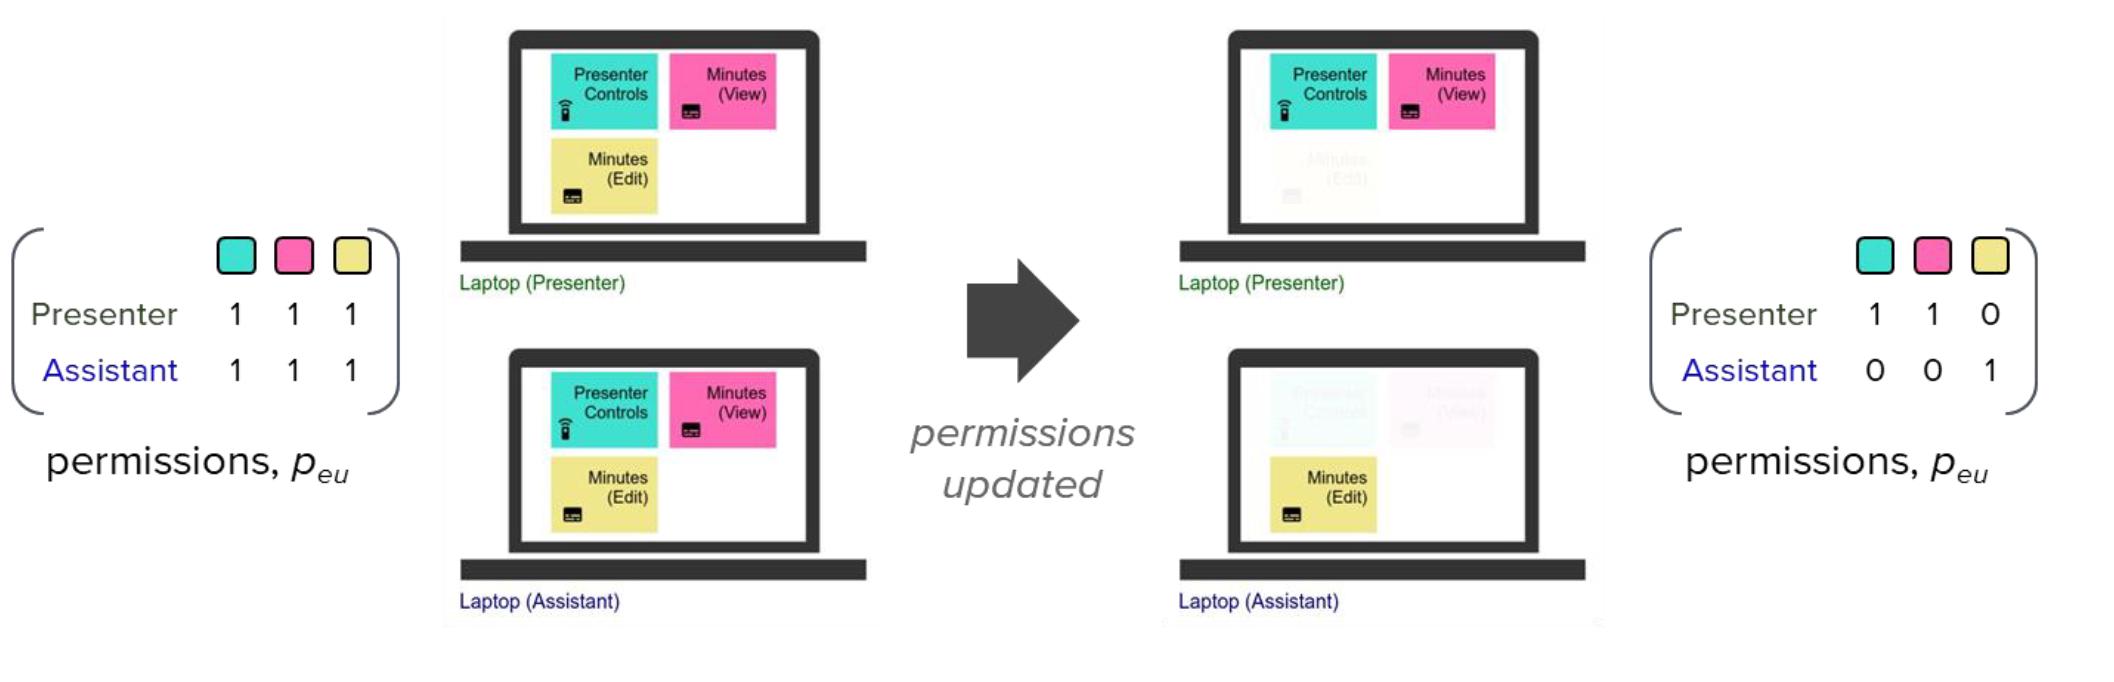
\includegraphics[width=\linewidth]{user_roles.png}
\end{center}

\textit{Cognitive Load}

\begin{center}
	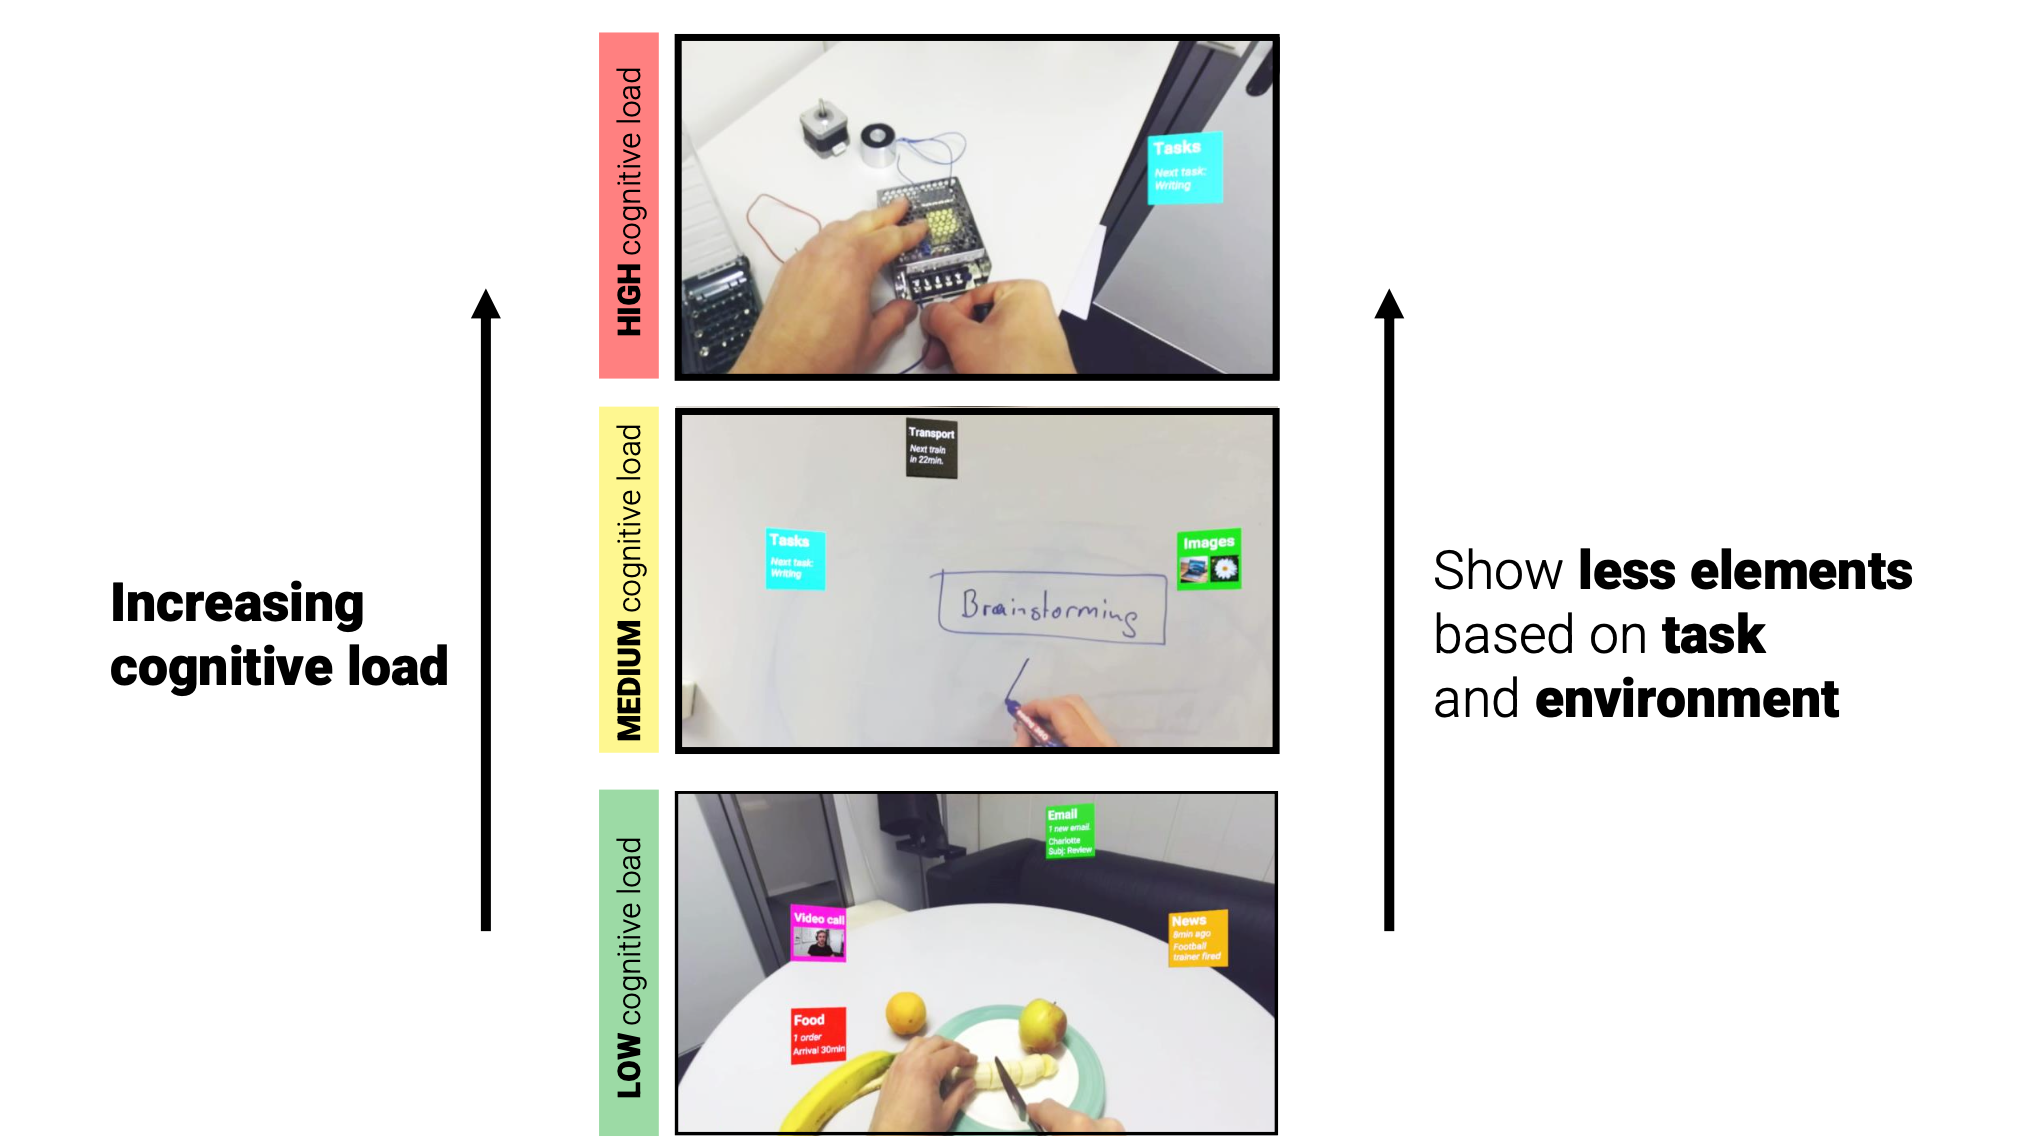
\includegraphics[width=\linewidth]{optimize_for_cognitive_load.png}
\end{center}


The idea then is to include cognitive load, cognitive capacity and cognitive cost to the objective function. \medskip

\textit{Optimize for environment} \smallskip

The idea is to optimize for differenct environments, e.g. screen placement, number or virtual screens etc. 
We include interaction modality, occlusion avoidance and temporal consistency in to the objective function. \smallskip

This can be done through assigning voxel containers to objects and surfaces. The objective would the be to optimally assign elements to containers. 

$x_{e,c} = \begin{cases} 1, & \text{if } e \text{ is assigned to } c \\ 0, & \text{otherwise} \end{cases}$

\begin{center}
	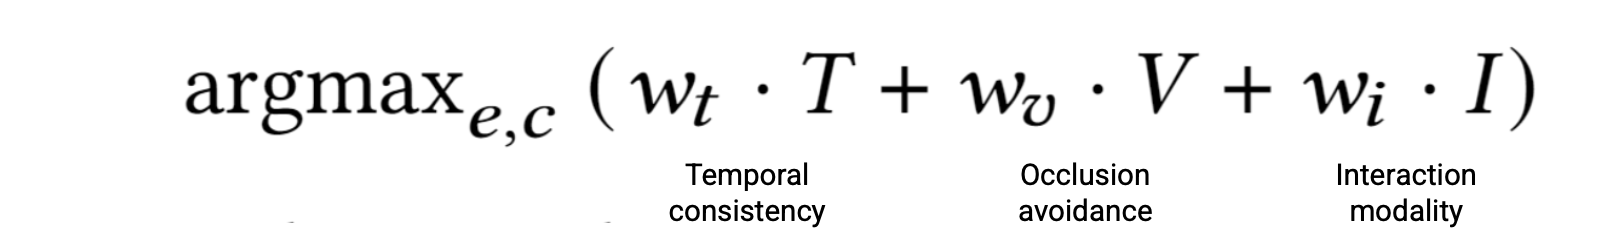
\includegraphics[width=\linewidth]{environment_formula.png}
\end{center}

\begin{center}
	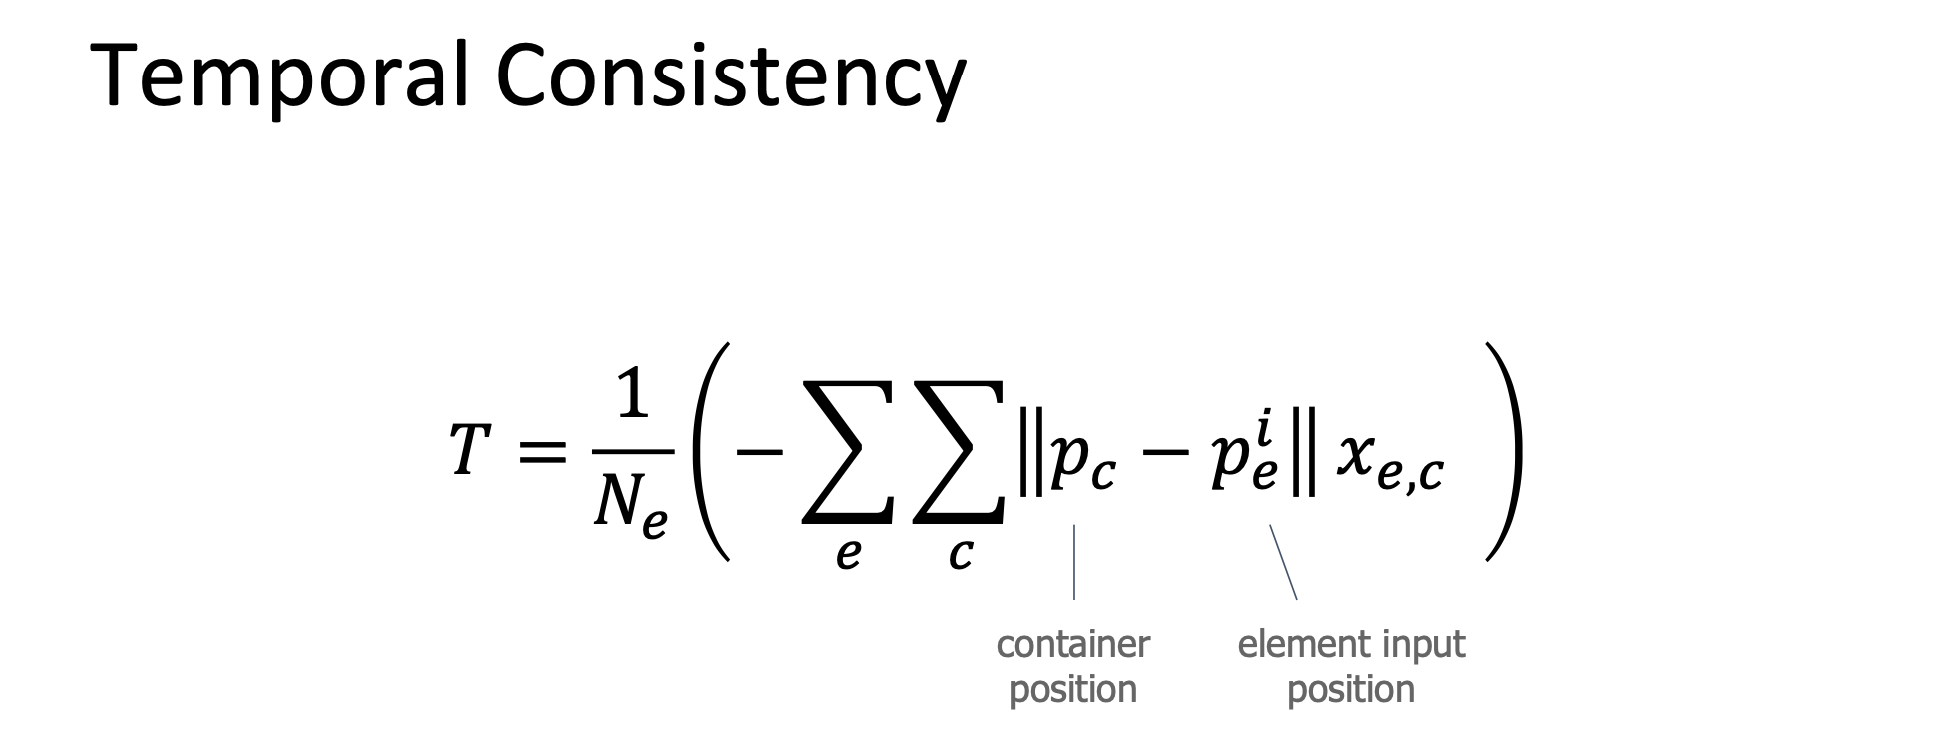
\includegraphics[width=\linewidth]{temporal_consistency.png}
\end{center}


\begin{center}
	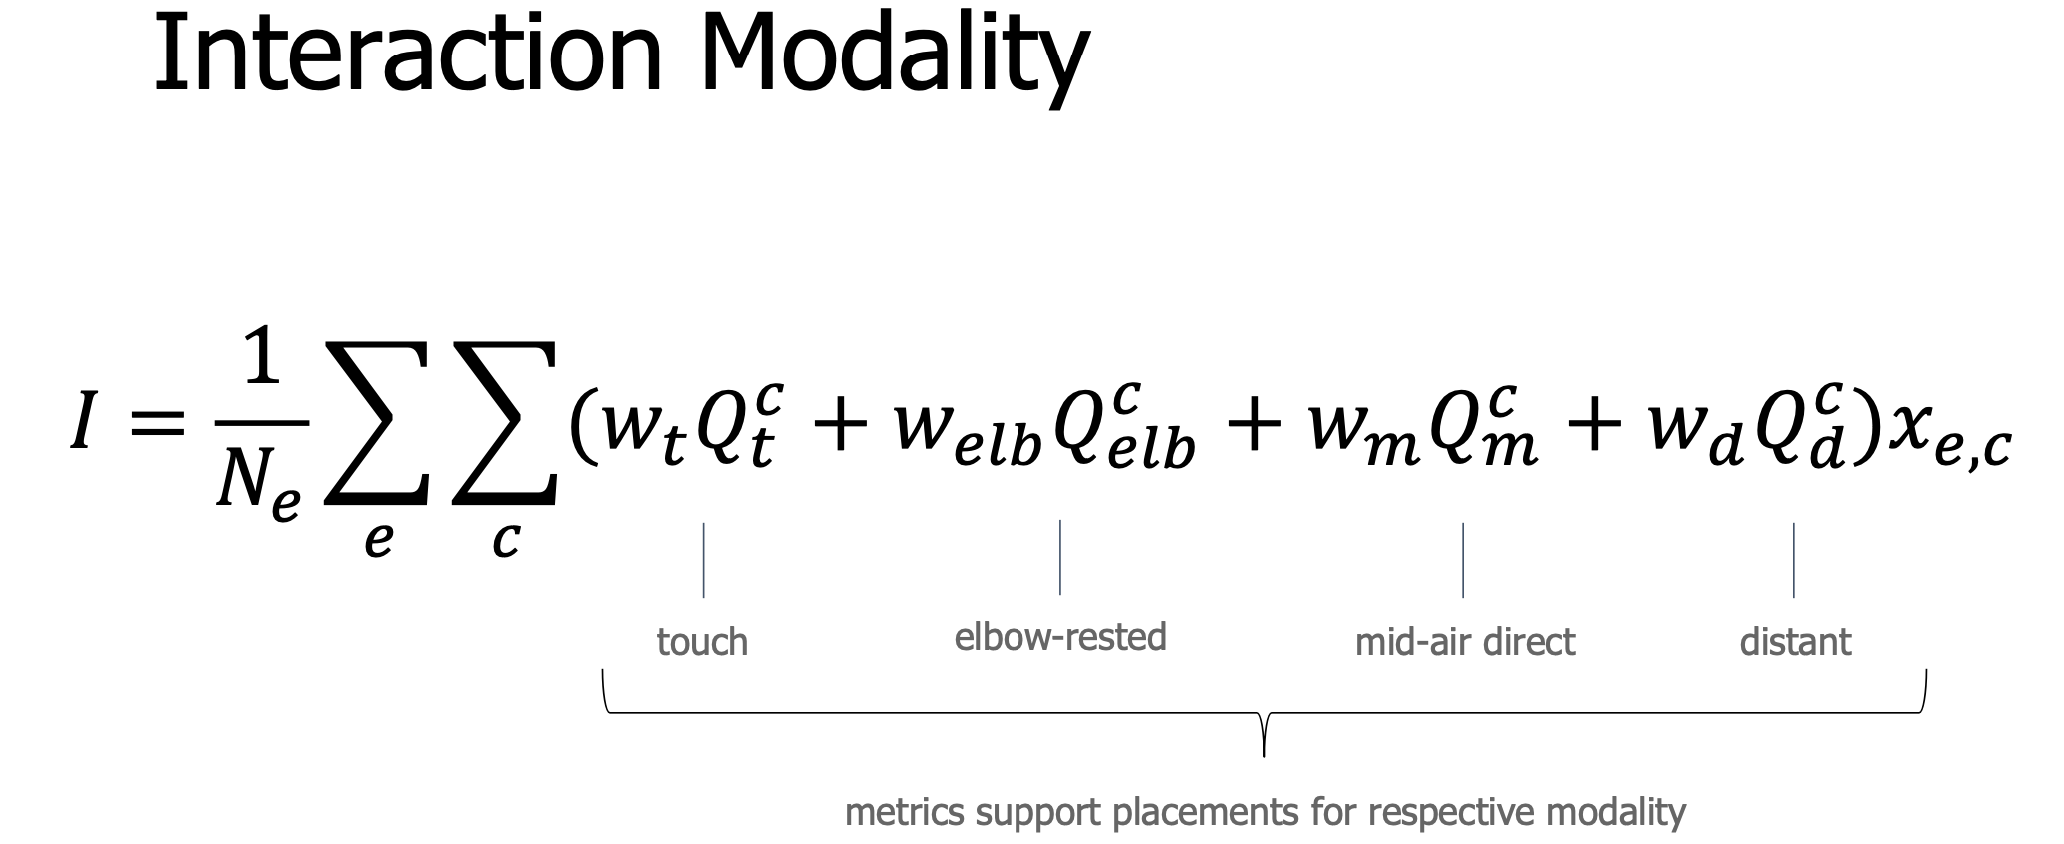
\includegraphics[width=\linewidth]{interaction_modality.png}
\end{center}

New contexts might introduce physical constraints that may render prior interface layouts unuseable. 

\columnbreak






